\part{Analysis}
\textit{Results from the implementation}
%present the details of the experiments
%   i. Hardware and Software info
%  ii. NN implementations : challenges in developing model & build for target HW
% iii. Different performance measurements: Training time, Model accuracy, Peak 	%	   memory utilised and memory footprint
%  iv. 


The HDR-NN training implementations were benchmarked on the iMX6SDB evaluation board. Model accuracy, execution time and peak memory utilised during the training of the model is compared while varying the number of layers and the neurons in each layer

\chapter{Results}
%Ideas: 1. Coefficient of variation
%		2. optimisation flags
%		3. Measurements using different tools 
%		4. Early stopping
%		5. Choosing Model parameters
%		6. Extrapolation

\section{HDR-NN comparisons}

The execution times for HDR-NN training were recorded for different network configurations such as differing hidden layer sizes of 2, 8, 32, and 128. The run times increased exponentially with the number of parameters. This is due to the fact that the amount of calculation in a fully connected network increases with the number of neurons, leading to longer training times

Further, when the number of neurons in a single layer exceeds 32, the accuracy of the model is observed to decrease due to overfitting. To improve accuracy, adding another layer with 16 neurons is found to be beneficial without significantly increasing the time required for computation. In fact, for larger network sizes, it is observed to even reduce the computation time required

Regardless of the hidden layer sizes, the peak memory utilisation remains constant for the same application regardless of the network configuration

\begin{figure}[ht]
	\centering
	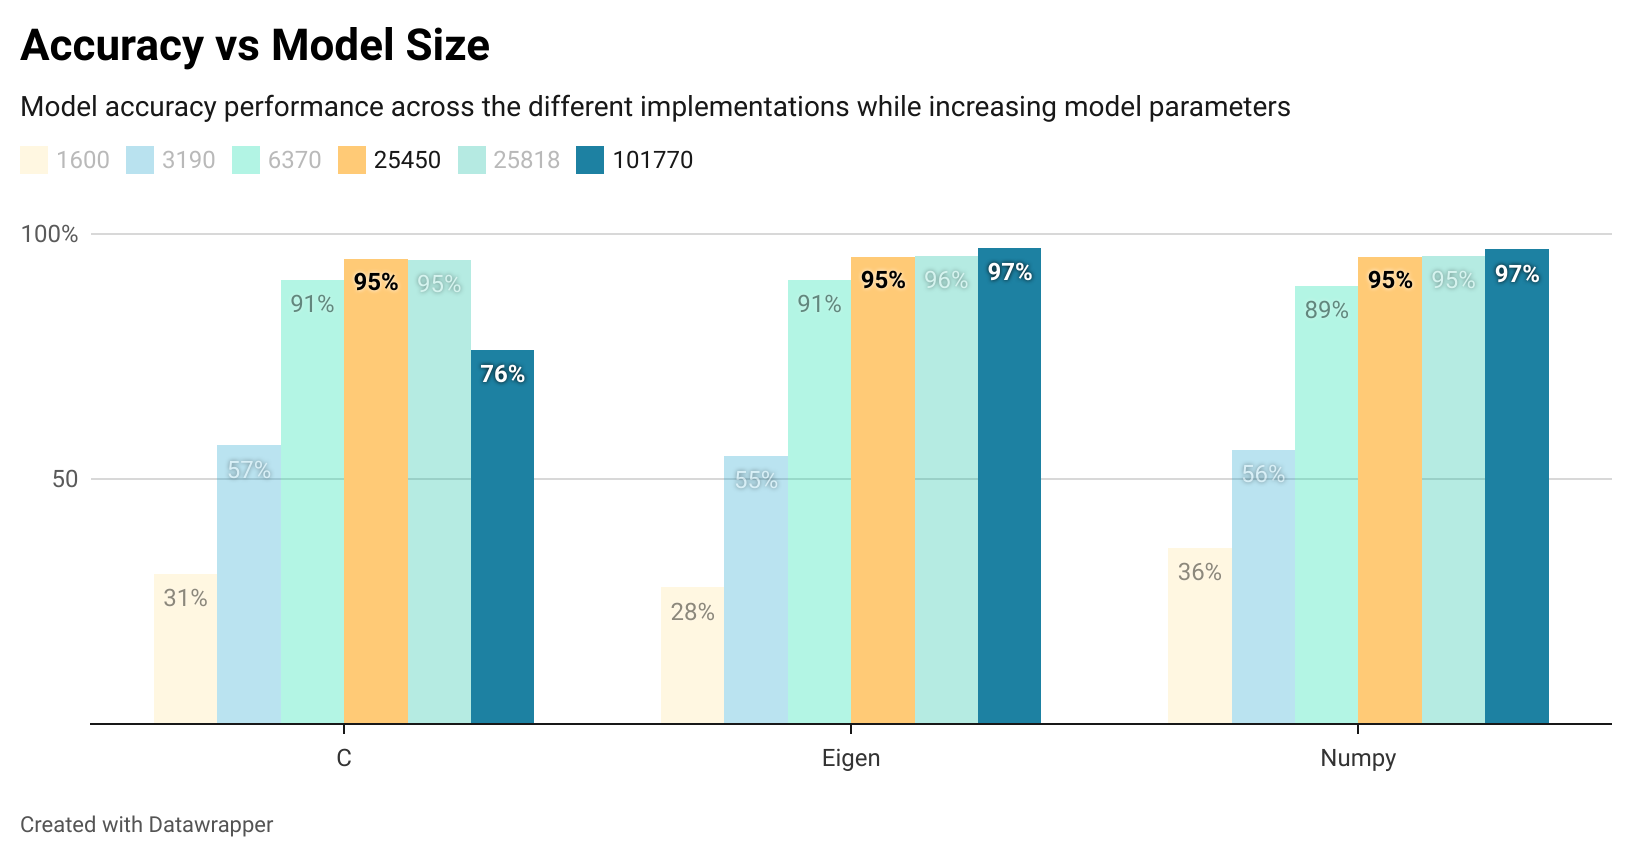
\includegraphics[scale=0.17]{accuracy}
	\caption[HDR-NN Accuracy]{Comparing the accuracy of the different HDR-NN implementations}
\end{figure}

\begin{figure}[ht]
	\centering
	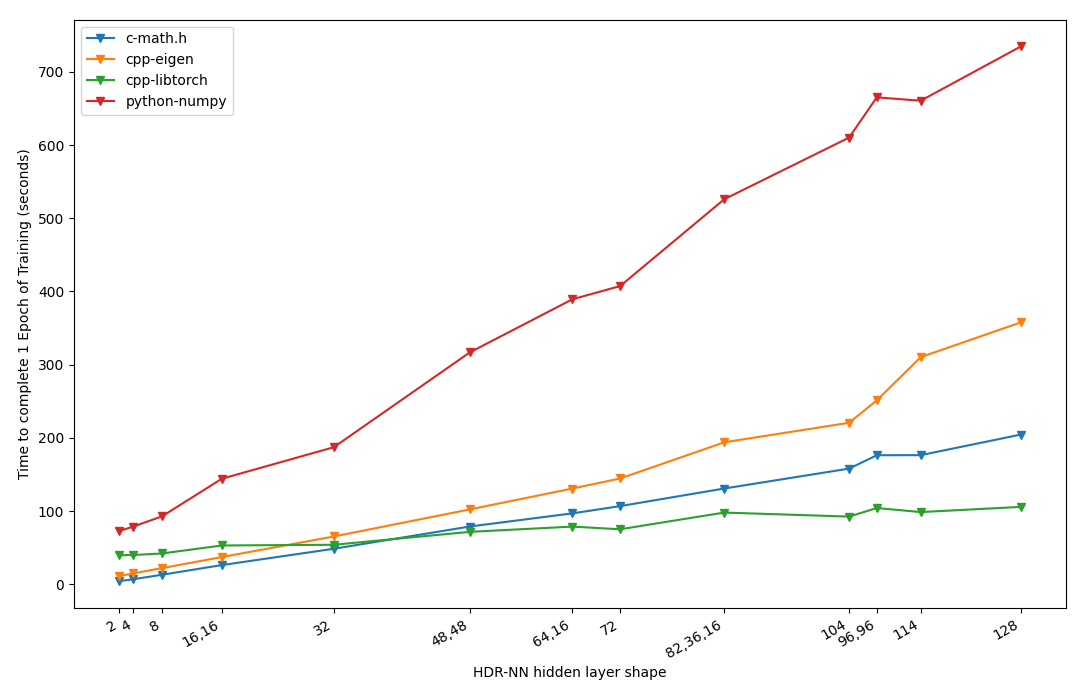
\includegraphics[scale=0.19]{exec-time}
	\caption[Execution Time vs Model Parameters]{Comparing total run time for training the different HDR-NN programs}
\end{figure}

\begin{figure}[ht]
	\centering
	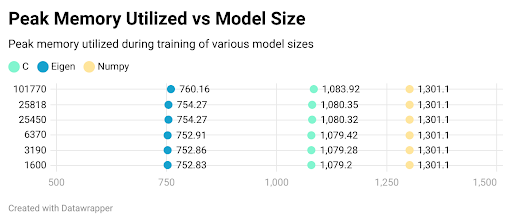
\includegraphics[scale=0.21]{memory-bar}
	\caption[Peak Memory Utilisation]{Peak Memory Utilized during training with different model sizes remain similar within the same implementation}
\end{figure}

\subsection[Python - Numpy]{Python Numpy based HDR-NN}

The Numpy implementation consistantly took longer duration to perform the same training cycle as compared to the C implementation

\subsection[Tensorflow Lite]{Tensorflow-Lite based HDR-NN}
\textit{Benchmark pending \dots}

\subsection[C]{C based HDR-NN}

C implementation had lower execution times and memory usage

\subsection[CPP - Eigen]{CPP based HDR-NN}
\textit{Benchmark pending \dots}

\section{CMSIS-NN based Optimisations to Training}
\textit{Further breakdown of the performance achieved from different optimisation techniques}

\subsection{Quantisation}
\textit{future: Training Network with Quantized weights}

\subsection{Pruning the Network}
\textit{future}

\chapter{Discussion}

\section{Developer Experience}

\chapter{Conclusion and Future Work}
\textit{What does it all mean? Where do we go from here?}
